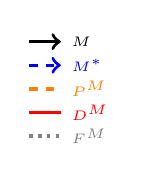
\begin{tikzpicture}[
very thick, 
->, 
every pin edge/.style={
	-, 
	very thin,
	decorate,
	decoration={snake},
	black!60,
}]
% \draw [help lines] (0,0) grid (3,2);

\tikzset{
	opt/.style={blue, dashed},
	d/.style={red, -},
	p/.style={orange, dashed,-},
	f/.style={gray, dotted,-},
}

\draw[] (3,1.3) -- (3.4,1.3) node[right]{\tiny $M$};
\draw[opt] (3,1) -- (3.4,1) node[right]{\tiny $M^*$};
\draw[p] (3,.7) -- (3.4,.7) node[right]{\tiny $P^M$};
\draw[d] (3,.4) -- (3.4,.4) node[right]{\tiny $D^M$};
\draw[f] (3,.1) -- (3.4,.1) node[right]{\tiny $F^M$};

% \graph[default graph]{
% 	{[nodes={d}]	3[x=0,y=0, pin=above right:{\small 2\$}],7[pin=below right:{\small 2\$}]};
% 	{[nodes={p}]	1[pin=above left:{\small 1\$}],2[pin=right:{\small 1\$}],4[pin=left:{\small 1\$}],5[pin=right:{\small 1\$}]};
% 	{[nodes={f}]	8,9,10};
% 	
% 	{1, 2} -> 3;
% 	{4, 5} -> 7;
% 
% 	{[edges={opt}]
% 	{1} -> 4;
% 	{8,9} -> 7;
% 	{2,3,10} -> 5;
% 	}
% };

\end{tikzpicture}